\chapter[Exploration Round 5 - Cantibox]{Exploration Round 5\\Cantibox}
\label{chapter:exploration-round-5}

\section{Goal}
\label{section:exploration-5-goal}

The robotic assembly process has already achieved a high degree of automation by the end of last round. The only exceptions are caused by alignment problems that cannot be resolved with the current robotic setup. The study was therefore expanded to integrate cutting-edge design methods with collaborators in two different fields. 

\begin{itemize}
	\item \textbf{Structurally-informed joint design --} Structural analysis and design using a novel method that is based on the theory of plasticity.%
    \footnote{The method is developed by Davide Tanadini. For details of the collaboration, see \noseeref{section:methodology-collaborations}.}
    This allows individually customised joints to respond to local load conditions. The main challenge on my part was to negotiate the intersection between assembly limitations, Computer Numeric Control (CNC) machining limitations and structural optimization. 

	\item \textbf{Automated Task and Motion Planning (TAMP) --} Performing TAMP in unison (instead of task planning before motion planning) using PDDLStream.%
    \footnote{The method is developed by Yijiang Huang and Caelan Garrett. For details of the collaboration, see \noseeref{section:methodology-collaborations}.}
    This allows for the optimisation of redundant tasks and robotic motions \seeref{subsection:exploration-2-joints-loosening-after-assembly}. The main challenge is to formulate actions that can be understood by the computer algorithm to plan automatically. 

\end{itemize}
The two technology was validated with the assembly of a structure consisting of three volumetric modular boxes. The structure is designed with lap joints that are assembled with clamped and screwed techniques that have been demonstrated in previous Exploration Rounds \seerefii{subsubsection:exploration-2-syncronous-movement-of-clamp-and-robot}{subsubsection:exploration-4-screwdriver-joint-closure}. The main differences in this assembly process are:

\begin{itemize}
	\item Combined operation of Clamps and Screwdrivers in one structure
	\item The largest amount of tools being used by the robotic assembly process so far
	\item Stability-aware design approach with scaffolding (instead of using redundant elements)
	\item Extending the camera vision alignment approach to attaching clamps on beam
\end{itemize}

This new attempt further validate the flexibility and modularity of the DiRT concept. It demonstrated that different tools can be chosen for a specific element depending on the joint design.%
\todo{Paragraph below rewritten to explain the benifit of combining clamped and screwed joint}
Compared to the unselective use of screwed joints everywhere in the HyparHut \seeref{subsubsection:exploration-4-fastener-kept-joints-from-loosening}, the demonstrator in this round was structurally analysed to determined which joints are prone to loosening.
Only those that demand fastening were designed with a left-in fastener \seeref{subsection:exploration-5-demonstrator-design-cantibox-pavilion}. This is a crucial step to demonstrate that a fabrication process can accommodate different performance-driven structural designs.

\subsection{Combined Operation of Clamps and Screwdrivers}
\label{subsection:exploration-5-combined-operation-of-clamps-and-screwdrivers}

\todo{Paragraph below also help explain the pros and cons of clamped and screwed joint}
There are different benefits and implications of using clamped joints versus screwed joints. For example, clamped joints are faster to assemble and the joint details are faster to machine, however, it is prone to loosening. The screwed joints can accomodate non-planar lap joints and are more stable after assembly, however, it is slower to assemble and require a speciality fastener. As the technology progress, it is likely to have more types of joints and tools to choose from. The assembly process should be able to accommodate different types of joints and tools in the same structure.

Figure \ref{fig:flowchart-for-combined-operation} shows the task planning flow chart for the combined operation of the Clamps and Screwdrivers. It is the result of merging the two previous flow charts \seerefii{subsubsection:exploration-3-task-planning-with-flowchart}{subsection:exploration-4-flowchart-for-screwdriver-assembly}.

\begin{figure}[!h]
    \centering
    \includegraphics[width=0.99\textwidth]{images/08/flowchart-3.pdf}
    \caption{Flowchart for combined operation of Clamps and Screwdrivers}
    \label{fig:flowchart-for-combined-operation}
\end{figure}


This method of merging flowcharts can become tedious as the number of tools increases.
\todo{Paragraph changed to clarify whether that the flowchart method is no longer used in this round.}
It is also not a very efficient way to plan tasks \seeref{subsection:exploration-5-tamp-with-pddlstream}. Therefore, the task planning method used in this exploration round will utilise a bottom-up planning method instead of the flowchart method \seeref{subsection:exploration-5-specifying-actions-and-goals-for-tamp-with-pddlstream}.

\section{Background}
\label{section:exploration-5-background}

\subsection{Structure and Joint Design Informed by Structural Analysis}
\label{subsection:exploration-5-structure-and-joint-design-informed-by-structural-analysis}

Historically, timber structures and joint details were designed based on the experience and intuition of skilled craftsmen, and their designs could only be tested empirically. As a result, the evolution of timber structures was slow, with only incremental changes being made over time. Timber material presents unique challenges for structural analysis due to its anisotropic and nonelastic behaviour, which require complicated computational models. 

Metallic connections elements are predominant in existing timber construction standards. For example, in the Swiss code SIA 265, only one timber-to-timber connection is described for new constructions. In the construction industry, timber-to-timber connections are mainly adopted in non-standard projects with rather generous budgets for extensive testing. For example, the Tamedia Building by the architect Shigeru Ban in Zurich (2013), where timber-to-timber joints were adopted to connect columns and beams. \parencite{tanadiniAnalysisDesignTimbertotimber2021}

Existing research on timber-to-timber connections is mostly related to the restoration of traditional timber roofs. For example, calculation procedures have been developed for the structural analysis of specific typologies of connections \parencite{holzerstefanm.StaticAssessmentHistorical2015}. However, the structural analysis of novel timber-to-timber connections remains challenging \parencite{tanadiniAnalysisDesignTimbertotimber2021}, as existing static calculation procedures are applicable only to single applications \parencite{fangJoineryConnectionsTimber2018, nguyenDevelopmentSpringModel2018, rezaeiradMacroscopicModelSpatial2020}. 

While this thesis does not specifically focus on computational engineering methods, it is important to ensure that the assembly method proposed in this thesis is compatible with ongoing development in the structural design field.

\subsection{TAMP with PDDLStream}
\label{subsection:exploration-5-tamp-with-pddlstream}

Task and Motion Planning (TAMP) with PDDLStream \parencite{garrettPDDLStreamIntegratingSymbolic2020} is a more advanced planning workflow that can create a more optimised task list than using the flowchart method. PDDLStream is an extension of the Planning Domain Definition Language (PDDL) that integrated sampling procedures with symbolic planning process.

In the previous planning workflow \seeref{subsection:exploration-3-process-design-workflow} tasks were planned using the flowchart method \seeref{subsubsection:exploration-3-task-planning-with-flowchart} without considering the geometrical constraints, such as reachability and collision. Motion planning happens only at a later stage with the already fixed task list. 

In a TAMP workflow, the tasks and motions are planned at the same time. This allows the geometrical constraints that are detected by the motion planner to be used as feedback for planning a different, and potentially more optimised, task sequence. However, in order to let the computer decide on the task list automatically, it is necessary to give it the freedom to compose tasks in different sequences. 

In contrast, the flowchart method can be seen as a top-down decision-making logic that has fixed the sequence of tasks. In other words, using the flowchart method will only lead to one deterministic task list with no freedom to try anything different. One of the apparent downsides of using the flowchart method was the inability to make a good long-term plan (also known as long-horizon plan). For example, in the previous clamped operation in Exploration Round 3, the used clamps were always retrieved from the structure back to the storage (Figure \ref{fig:photo-clamps-operation-round-3}). This was the only way to ensure that the clamp could still be accessible by the robot at a later step for a different beam in the assembly process. 

\begin{figure}[!h]
    \centering
    \includegraphics[width=0.99\textwidth]{images/08/img02.jpg}
    \caption{Photo showing clamps operation in Exploration Round 3}
    \label{fig:photo-clamps-operation-round-3}
\end{figure}


If a conditional logic is used in the flowchart to leave the clamp on the structure and retrieve it later, it can run into the inaccessible problem mentioned before. The motion planner will never be able to plan pass the inaccessible situation, causing the entire task plan to be \textit{stuck}. This problem is analogous to a game of chess where a player makes a series of moves that result in a checkmate with no way out. The player is forced to either concede defeat or re-evaluate their strategy and backtrack to avoid the hopeless situation.

By employing the TAMP workflow using PDDLStream, the solver has the ability to backtrack and explore a different task sequence. For example, by choosing to move the clamp earlier, or to move the clamp back to storage after use. This adaptable and intelligent approach to planning assembly tasks can potentially lead to more efficient and optimised robotic operations.

\section{Development}
\label{section:exploration-5-development}

\subsection{Structurally Informed Polyline Lap Joint}
\label{subsection:exploration-5-structurally-informed-polyline-lap-joint}

In order to study the integration with an analysis-driven joint design process, a design workflow was created to incorporate a newly developed joint design method that is based on the theory of plasticity \parencite{tanadiniLimitAnalysisTimber2023}. Figure \ref{fig:workflow-for-structural-checks} shows the workflow of the design process where global structural behaviour and assemblability were checked during the design process to create a global arrangement of beams (the Assembly Model). FEA was performed on the global level to compute the forces that are experienced by the joint. 

Joint design is a human-in-the-loop process that is assisted by a computer simulation tool. The geometry of the joint was adjusted by controlling the proportions of the joint such that the stresses do not exceed the yield condition of the material.

\begin{figure}[!h]
    \centering
    \includegraphics[width=0.99\textwidth]{images/08/structural-checks.pdf}
    \caption{Workflow for structural checks during joint design}
    \label{fig:workflow-for-structural-checks}
\end{figure}


The polyline lap joint was used as the parametric model that describes a design space \seeref{subsection:exploration-4-parametric-polyline-lap-joints}. Fabrication checks were performed during the joint design process to ensure that the results did not violate the 90-degree rule \seeref{subsection:exploration-4-cnc-limitation-in-cutting-lap-joints}. 

Figure \ref{fig:ui-contact-surface} shows how the polyline lap joint parametric model is decomposed into different contact areas for analysis. Each area contributes to a different force transfer resistance depending on its location and angle. The controls used for adjusting the joint geometry can be seen in the Grasshopper interface. The fabrication check can be seen returning an ``OK" message. Figure \ref{fig:ui-polyline-lap-joint} shows a different interface that focused on the design of the polyline lap joint. Angle check for CNC fabrication is also integrated into the same interface. 

\begin{figure}[!h]
    \centering
    \includegraphics[width=0.99\textwidth]{images/08/img04.png}
    \caption[User interface for analysing contact surfaces in a polyline lap joint]
    {User interface for analysing contact surfaces and reaction forces in a polyline lap joint using force and form diagram} {\footnotesize (Credit: Diagram by Davide Tanadini \parencite{tanadiniLimitAnalysisTimber2023})}
    \label{fig:ui-contact-surface}
\end{figure}

\begin{figure}[!h]
    \centering
    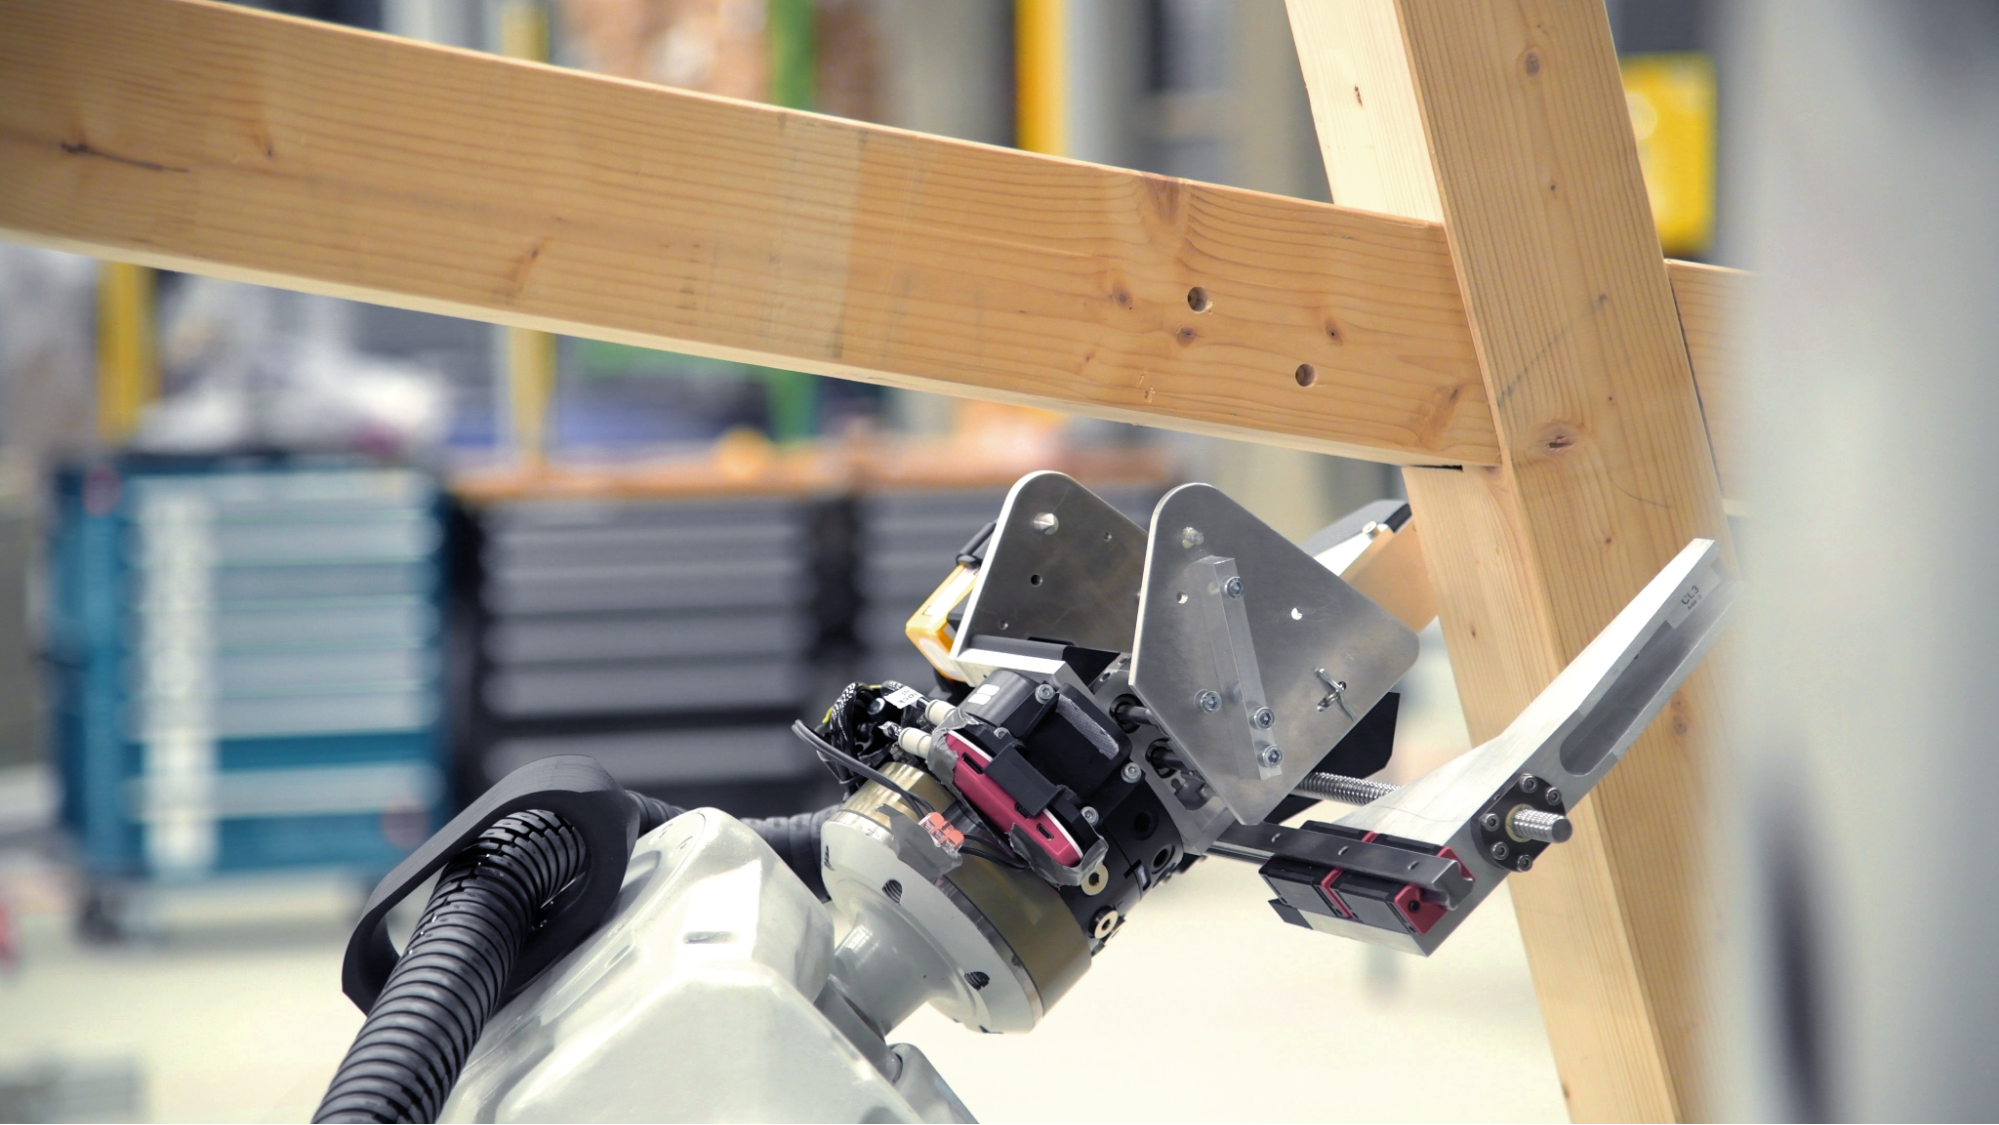
\includegraphics[width=0.99\textwidth]{images/08/img05.png}
    \caption[User interface for designing polyline lap joints]
    {User interface for designing polyline lap joints, combining structural and fabrication check} {\footnotesize (Credit: Diagram by Davide Tanadini \parencite{tanadiniLimitAnalysisTimber2023})}
    \label{fig:ui-polyline-lap-joint}
\end{figure}


Figure \ref{fig:customised-joints} shows some of the customised joints used in the demonstrator.
\todo{Pointed readers to Davide's thesis for details how the joints are designed.}
The shape of the joints all share the same parametric model but have different parameters depending on the local load conditions. For details regarding how the joints are designed, refer to Tanadini \parencite*{tanadiniLimitAnalysisTimber2023}.

% 2 x 2 Images
\begin{figure}[!h]
    \centering
    \begin{subfigure}[b]{0.49\textwidth}
        \centering
        \includegraphics[width=\textwidth]{images/08/img06.jpg}
        % \caption{SubFigureCaption}
        %\label{fig:uniquesubfigurelabel}
    \end{subfigure}
    \hfill
    \begin{subfigure}[b]{0.49\textwidth}
        \centering
        \includegraphics[width=\textwidth]{images/08/img07.jpg}
        % \caption{SubFigureCaption}
        %\label{fig:uniquesubfigurelabel}
    \end{subfigure}
    \vskip\baselineskip % Next row
    \begin{subfigure}[b]{0.49\textwidth}
        \centering
        \includegraphics[width=\textwidth]{images/08/img08.jpg}
        % \caption{SubFigureCaption}
        %\label{fig:uniquesubfigurelabel}
    \end{subfigure}
    \hfill
    \begin{subfigure}[b]{0.49\textwidth}
        \centering
        \includegraphics[width=\textwidth]{images/08/img09.jpg}
        % \caption{SubFigureCaption}
        %\label{fig:uniquesubfigurelabel}
    \end{subfigure}
    \caption{Examples of customised joints used in the demonstrator}
    \label{fig:customised-joints}
\end{figure}


\subsection{Scaffolding Support During Assembly}
\label{subsection:exploration-5-scaffolding-support-during-assembly}

The principles of deformation-aware design \seeref{subsection:exploration-4-deformation-awareness-and-error-correction-by-triangulation} was used to design the structure, specifically for the identification of high-risk elements. 
\todo{The paragraph is reworded for better language}
However the approach of adding diagonal bracing to the structural system \seeref{subsubsection:exploration-4-global-correction-approach} is not used, because it would defeat the purpose of the reciprocal structural concept. Therefore, temporary scaffolding was used instead to create stable structural triangles during assembly to stablize the structure. 

The temporary scaffoldings are made from aluminium profiles, each of them consists of three hinged segments. The middle segment is the longest portion that acts at one of the rigi triangle sides, while the two segments at the ends provide clamping surfaces between the timber structure and the scaffolding. Figure \ref{fig:photo-scaffolding-support} shows one end of the scaffolding, the short segments can be clamped to the timber structure using a carpentry clamp.

\begin{figure}[!h]
    \centering
    \includegraphics[width=0.99\textwidth]{images/08/img10.jpg}
    \caption{Photo showing scaffolding support during assembly}
    \label{fig:photo-scaffolding-support}
\end{figure}



In order to avoid collision during the robotic operation \seeref{subsection:exploration-3-robot-collision-with-scaffolding}, the estimated size of the scaffolding bar and the carpentry clamps are added to the 3D model as collision geometry for motion planning.

Figure \ref{fig:cm-scaffolding-bars} shows the collision geometry of the scaffolding bars (yellow) in the Process Model. \todo{Added clarification sentence to explain how the collision model is created}The collision geometry and their order of appearance in the assembly sequence is added by the Process Engineer during process design stage. During the task planning, this is treated as an element that is assembled manually. Hence they also contain a sequence number. During construction they are assembled by the operator after the unstable beam is clamped and before the robot gripper lets go of it. 


\begin{figure}[!h]
    \centering
    \includegraphics[width=0.99\textwidth]{images/08/img11.jpg}
    \caption{Collision geometry of scaffolding bars in Process Model}
    \label{fig:cm-scaffolding-bars}
\end{figure}

\subsection{Automatic Shake when Docking with Tools}
\label{subsection:exploration-5-automatic-shake-when-docking-with-tools}

After the implementation of the vision-guided docking procedure \seeref{subsection:exploration-4-camera-marker-hardware-on-docking-adapter} and the compliant robotic arm control \seeref{subsection:exploration-4-compliant-control-for-robotic-arm}, there are still cases where the docking adapter failed to lock \seeref{subsection:exploration-3-docking-adapter-fail-to-lock}.

In the last demonstration, the operator found that it was possible to fix the problem remotely by jogging the gantry linearly back and forth, while keeping the robotic arm in a low-stiffness model. 

In this exploration round, a shaking routine was developed to automatically perform the jogging movement whenever the docking switches did not return a locked signal.
\todo{Added mention of the success rate}
The routine would later prove to solve more than 80\% of the locking failure. The following pseudocode describes the procedure:

\begin{description}[nosep]
    
	\item[Step 1] Check lock signal
    \begin{enumerate}
        \item If the lock signal is not acquired
        \begin{enumerate}
            \item If attempt\_count $<$ 5, go to step 2
            \item If attempt\_count $\geq$ 5, exit and report a failed docking lock.
        \end{enumerate}
        \item If the lock signal is acquired, exit and report a successful lock
    \end{enumerate}

	\item[Step 2] Perform a shake with a predefined speed and movement distance
    \begin{enumerate}
        \item Shake X axis, and then Y axis, and then Z axis

        \begin{enumerate}
            \item Move the axis, towards the positive direction
            \item Move the axis, towards the negative direction
            \item Go back to original point
        \end{enumerate}
    \end{enumerate}

	\item[Step 3] Increase shaking speed and movement distance and go to step 1
\end{description}

\subsection{Camera-Marker Hardware on CL3 Clamp}
\label{subsection:exploration-5-camera-marker-hardware-on-cl3-clamp}

Following the success of the vision-guided docking, the same principle is applied to the attachment of the clamps to the beams. The difference is that the cameras will not be installed inside the body of the CL3 clamp (a retrofit) and the markers have to be attached to the beams. The images below show the intended location of the camera and the marker in the alignment position before attaching the clamp to the beam.

% 2 Horizontal Image  
\begin{figure}[!h]
    \centering
    \begin{subfigure}[b]{0.49\textwidth}
        \centering
        \includegraphics[width=\textwidth]{images/08/img12.jpg}
        % \caption{SubFigureCaption}
        %\label{fig:uniquesubfigurelabel}
    \end{subfigure}
    \hfill
    \begin{subfigure}[b]{0.49\textwidth}
        \centering
        \includegraphics[width=\textwidth]{images/08/img13.jpg}
        % \caption{SubFigureCaption}
        %\label{fig:uniquesubfigurelabel}
    \end{subfigure}
    \caption{Diagram showing the relative position of camera on CL3 Clamp and marker on beam}
    %\label{fig:uniquefigurelabel}
\end{figure}


Figure \ref{fig:esp32-cam-board-in-case} shows the ESP32 CAM board in a custom 3D-printed enclosure without the cover. Figure \ref{fig:four-camera-assemblies-constructed} shows the four camera assemblies installed in the clamps. The power cables and WiFi antenna cables can be seen coming out of the enclosure. Notice the two symmetrical designs, they are for the CL3 and CL3M clamps. Figure \ref{fig:camera-assembly-inside-a-cl3-clamp} shows the camera assembly installed inside the gripper of a CL3 Clamp. 

% 2 Horizontal Image  
\begin{figure}[!h]
    \centering
    \begin{subfigure}[b]{0.49\textwidth}
        \centering
        \includegraphics[width=\textwidth]{images/08/img14.jpg}
        \caption{Prototype enclosure for the camera}
        \label{fig:esp32-cam-board-in-case}
    \end{subfigure}
    \hfill
    \begin{subfigure}[b]{0.49\textwidth}
        \centering
        \includegraphics[width=\textwidth]{images/08/img15.jpg}
        \caption{Four camera assemblies constructed}
        \label{fig:four-camera-assemblies-constructed}
    \end{subfigure}
    \caption{Photos of the constructed camera assemblies}
    %\label{fig:uniquefigurelabel}
\end{figure}

\begin{figure}[!h]
    \centering
    \includegraphics[width=0.99\textwidth]{images/08/img16.jpg}
    \caption{Photo of camera assembly installed inside a CL3 Clamp}
    \label{fig:camera-assembly-inside-a-cl3-clamp}
\end{figure}


Figure \ref{fig:calibration-setup-for-camera-assembly} shows the clamp being calibrated with a calibration jig. The jig positioned a marker accurately at a location where it would be found on the timber beams. Figure \ref{fig:wifi-antenna-on-clamp} shows the position where the WiFi antenna is taped to the bottom of the clamp.

% 2 Horizontal Image  
\begin{figure}[!h]
    \centering
    \begin{subfigure}[b]{0.49\textwidth}
        \centering
        \includegraphics[width=\textwidth]{images/08/img17.jpg}
        \caption{Calibration jig attached to a Clamp}
        %\label{fig:uniquesubfigurelabel}
    \end{subfigure}
    \hfill
    \begin{subfigure}[b]{0.49\textwidth}
        \centering
        \includegraphics[width=\textwidth]{images/08/img18.jpg}
        \caption{Calibration jig}
        %\label{fig:uniquesubfigurelabel}
    \end{subfigure}
    \caption{Photos showing how the camera installed inside the clamps can be calibrated using a jig}
    \label{fig:calibration-setup-for-camera-assembly}
\end{figure}

\begin{figure}[!h]
    \centering
    \includegraphics[width=0.99\textwidth]{images/08/img19.jpg}
    \caption{Photo showing the WiFi antenna at the bottom of a clamp}
    \label{fig:wifi-antenna-on-clamp}
\end{figure}

\FloatBarrier

The markers are made with a waterproof label that can be ink-jet printed. Figure \ref{fig:setup-for-placing-allignment-markers} shows a placement guide used to position the markers accurately on the beam by registering to the gripper hanging holes. Future work should consider printing or laser engraving the markers on the wood directly by attachments on the automatic joinery machines.

% 2 Horizontal Image  
\begin{figure}[!h]
    \centering
    \begin{subfigure}[b]{0.45\textwidth}
        \centering
        \includegraphics[width=\textwidth]{images/08/img20.jpg}
        \caption{Label placement guide}
        \label{fig:label-placement-guide}
    \end{subfigure}
    \hfill
    \begin{subfigure}[b]{0.53\textwidth}
        \centering
        \includegraphics[width=\textwidth]{images/08/img21.jpg}
        \caption{Operation of the placement guide}
        \label{fig:marker-placement-on-beam}
    \end{subfigure}
    \caption{Setup for placing allignment markers on the timber beams}
    \label{fig:setup-for-placing-allignment-markers}
\end{figure}

\subsection{Specifying Actions and Goals for TAMP with PDDLStream}
\label{subsection:exploration-5-specifying-actions-and-goals-for-tamp-with-pddlstream}

Task and Motion Planning (TAMP) with PDDLStream is a method for integrating high-level planning and low-level motion planning in a single, unified framework \seeref{subsection:exploration-5-tamp-with-pddlstream}. The approach enables the automatic generation of optimised task sequences, considering both abstract actions and their geometric constraints. 

In the implementation of this Clamped and Screwed Assembly Process, the abstract actions refer to the High-Level Tasks, identical to those used in the flow chart. They are defined as groups of Low-Level Tasks \seeref{subsubsection:exploration-3-expanding-task-groups}. The geometric constraints refer to the Inverse Kinematic (IK) check that ensures reachability. 

Here is a summary of how the TAMP is performed with PDDLStream:

\begin{itemize}
	\item \textbf{Problem Formulation --} Actions (High-level Tasks), initial state and goal state are represented in a symbolic form using the PDDL (Planning Domain Definition Language) syntax.

\begin{itemize}
	\item \textbf{Initial State --} Identical to the initial state used for sequential planning \seeref{subsubsection:exploration-3-compute-object-states}. All the state parameters of all objects are required.

	\item \textbf{Actions --} Actions consist of two parts. 

\begin{itemize}
	\item \textbf{Preconditions --} A symbolic criteria that the scene state must meet before the action can be taken. 

	\item \textbf{Effects --} A symbolic change to the scene state if that action is taken. This is conceptually the same as the \verb|task.UpdateState()| function \seeref{subsubsection:exploration-3-compute-object-states} but implemented for the High-Level Tasks.

\end{itemize}
	\item \textbf{Goal State --} The state of all objects which the planner will attempt to achieve. This refers to the state where all beams are assembled, and all tools are placed back at their storage location.

\end{itemize}
	\item \textbf{Stream Functions --} Stream functions are implemented that connect the actions to their geometric constraints. There is one stream Function for each robotic Action. They contain IK solvers that can check whether the targets in the High-Level Task are reachable.

\begin{itemize}
	\item IK solvers have access to the same Robot Model and Tool Models \seeref{subsection:exploration-3-process-design-workflow} for checking IK and collisions.

\end{itemize}
	\item \textbf{PDDLStream Integration} \textbf{-} The PDDL problem definition and the stream functions are integrated using PDDLStream. PDDLStream extends PDDL by allowing the integration of external procedures (stream functions) into the planning process.

	\item \textbf{Planning --} The PDDLStream planner was used to generate a sequence of high-level tasks while ensuring low-level motions are reachable. The planner explores different task sequences and backtracks automatically during the search. This results in a more efficient and optimised robotic operation while ensuring targets are reachable.

	\item \textbf{Motion Planning --} During the PDDLStream planning, only the IK result was checked. The motion planning between the targets was performed afterwards to find the trajectory that links between the targets.

	\item \textbf{Execution --} The execution of the planned tasks and motion on the robot is the same as before \seeref{subsection:exploration-3-standalone-process-execution-controller}. One side effect is that the planned tasks no longer correspond to a specific beam in a sequential way, but this does not affect operations.

\end{itemize}
\section{Demonstration}
\label{section:exploration-5-demonstration}

\subsection{Design Goal}
\label{subsection:exploration-5-design-goal}

\begin{itemize}
	\item Validate the assembly of structurally customised lap joints. Customization comes from structural analysis (work by Davide Tanadini)

	\item Exploring the design of a modular box typology that can be prefabricated and transported

	\item Designed to validate the use of scaffolding to improve stability

	\item Designed to use both Screwdrivers and Clamps in one structure

\begin{itemize}
	\item Three SL1 Screwdriver, One SL1\_G200 Screwdriver

	\item Two CL3 Clamp, Two CL3M Clamp

\end{itemize}
\end{itemize}

\FloatBarrier

\subsection{Design Team Information}
\label{subsection:exploration-5-design-team-information}

\begin{table}[!h]
    \includegraphics[page=1, trim=25.4mm 180mm 25.4mm 33mm, clip, width=0.98\textwidth]{tables/Tables in Chapter 8.pdf}
    \caption{Design Team Information for CantiBox Pavilion}
    % \label{table:LABELTEXT}
\end{table}

\FloatBarrier

\subsection{Demonstrator Design - CantiBox Pavilion}
\label{subsection:exploration-5-demonstrator-design-cantibox-pavilion}

CantiBox consists of three independent volumetric modules. Two modules are situated on the ground while the third central modules cantilevers on one side on top of the two other modules. Each unit is composed of 20 linear timber elements with a cross-section of 100mm x 100mm. Each face of the boxes is made of six timber linear elements (3 vertical and 3 horizontal) that are arranged in the plane to create a reciprocal system. 

\begin{figure}[!h]
    \centering
    \includegraphics[width=0.99\textwidth]{images/08/img22.jpg}
    \caption{Photo of the CantiBox Pavilion, after it is moved to the park}
    \label{fig:photo-cantibox-park}
\end{figure}

One element on each face behaves as the key element that closes the reciprocal system and interlocks the structure. Therefore, screwed joints are used on this key element, and all other joints are assembled by clamps without any fasteners. Figure \ref{fig:drawing-canitibox-pavilion} show the entire structure; the key elements are highlighted in blue; the dimension units are in mm. 

% 2 Horizontal Image  
\begin{figure}[!h]
    \centering
    \begin{subfigure}[b]{0.49\textwidth}
        \centering
        \includegraphics[width=\textwidth]{images/08/img23.jpg}
        \caption{Top View}
        %\label{fig:uniquesubfigurelabel}
    \end{subfigure}
    \hfill
    \begin{subfigure}[b]{0.49\textwidth}
        \centering
        \includegraphics[width=\textwidth]{images/08/img24.jpg}
        \caption{Front Elevation}
        %\label{fig:uniquesubfigurelabel}
    \end{subfigure}
    \caption{Drawings of the CantiBox Pavilion}
    \label{fig:drawing-canitibox-pavilion}
\end{figure}

Equilibrium-based methods and Finite Element Analysis (FEA) are used for the evaluation of the global structural behaviour of the CantiBox. In the analysis, each joint is regarded as a rigid connection. The self-weight of the structure and the wind load are taken into account. For each connection, the most disadvantageous load combination is considered. The capacity of linear timber elements to resist axial forces, shear forces, and bending moments is determined according to the Swiss code \parencite{swissstandardsassociationSIA265Timber2003}.

The pavilion is additionally furnished with a manually assembled floor system similar to the HyparHut, and a fabric covering for providing sun protection for occupants when the pavilion is moved to a nearby park. Figure \ref{fig:photo-cantibox-foundation} shows the pinned connection to the ground foundation. The foundation is an adjustable steel bracket that rests on top of the topsoil.

% 2 Horizontal Image  
\begin{figure}[!h]
    \centering
    \begin{minipage}[b]{0.68\textwidth}
        \centering
        \includegraphics[width=\textwidth]{images/08/img25.jpg}
        \caption{Photo showing the side of the CantiBox Pavilion}
        \label{fig:photo-cantibox-side}
    \end{minipage}
    \hfill
    \begin{minipage}[b]{0.3\textwidth}
        \centering
        \includegraphics[width=\textwidth]{images/08/img26.jpg}
        \caption{Photo showing the joint between the CantiBox Pavilion and the ground foundation}
        \label{fig:photo-cantibox-foundation}
    \end{minipage}
    % \caption{FigureCaption}
    %\label{fig:uniquefigurelabel}
\end{figure}

\subsection{Execution Preparation}
\label{subsection:exploration-5-execution-plan}

The preparation of the execution was similar to the previous round \seeref{subsection:exploration-4-execution-plan}. The aluminium platform was reused from the previous round. The main differences in the preperation are:

\begin{itemize}
	\item The taught configuration for the clamps are added for motion planning
	\item The test fit inspection discovered another type of inaccuracy \seeref{subsection:exploration-5-inaccurate-polyline-lap-problem}
	\item Robotic assembly is a combination of the clamped and screwed process \seerefii{subsection:exploration-5-combined-operation-of-clamps-and-screwdrivers}{subsection:exploration-5-specifying-actions-and-goals-for-tamp-with-pddlstream}
\end{itemize}

Figure \ref{fig:photo-clamps-and-screwdrivers} shows the tool storage location, which consists of 4 clamps and 4 screwdrivers. The storage pads for the clamps are different from the ones used in Exploration Round 3. These new ones have a top-facing flange direction that is easier for operator alignment.

\begin{figure}[!h]
    \centering
    \includegraphics[width=0.99\textwidth]{images/08/img27.jpg}
    \caption{Photo showing 4 clamps and 4 screwdrivers for the CantiBox Pavilion}
    \label{fig:photo-clamps-and-screwdrivers}
\end{figure}

The joints are chamfered in a similar way as before using a hand plane and chisel \seeref{subsection:exploration-2-clamping-joints-with-chamfered-edges}. The amount of chamfer was 6mm (Figure \ref{fig:joint-edge-chamfering}). However, the more complex polyline joint shapes made the manual process rather tedious. Figure \ref{fig:drilling-pin-gripper-holes} shows the pin gripper holes being drilled using the drilling jig \seeref{subsubsection:exploration-4-correction-of-the-screw-holes}.

% 2 Horizontal Image  
\begin{figure}[!h]
    \centering
    \begin{subfigure}[b]{0.49\textwidth}
        \centering
        \includegraphics[width=\textwidth]{images/08/img28.jpg}
        \caption{Joint edge chamfering}
        \label{fig:joint-edge-chamfering}
    \end{subfigure}
    \hfill
    \begin{subfigure}[b]{0.49\textwidth}
        \centering
        \includegraphics[width=\textwidth]{images/08/img29.jpg}
        \caption{Drilling pin gripper holes}
        \label{fig:drilling-pin-gripper-holes}
    \end{subfigure}
    \caption{Manual operation on the CantiBox beams before assembly}
    %\label{fig:uniquefigurelabel}
\end{figure}

\section{Lessons Learnt}
\label{section:exploration-5-lessons-learnt}

Note that this was the last exploration round. Any potential follow-up actions can only be pursued by future works.

\subsection{Successful Validation}
\label{subsection:exploration-5-successful-validation}

The pavilion was successfully constructed with a high degree of automation similar to the previous round. Apart from the inaccurately machined CNC joints and some episodic problems, the process went smoothly. 

Figure \ref{fig:photo-last-element-assembly} shows the last element being assembled for one of the three modules. The temporary scaffolding can be seen still attached inside the structure. 

\begin{figure}[!h]
    \centering
    \includegraphics[width=0.99\textwidth]{images/08/img30.jpg}
    \caption{Photo showing the assembly of the last element for one of the three modules}
    \label{fig:photo-last-element-assembly}
\end{figure}

\subsubsection{Stability from Scaffolding}
\label{subsubsection:exploration-5-stability-from-scaffolding}

Four temporary supports were planned for each of the modules, supporting each of the four columns at the corners. The use of scaffolding provided crucial stability for the partial structure during construction. The leaning columns would be extremely unstable and may even cause damage to the joint at the bottom if they would be unsupported. 

The task for the operator to attach the scaffolding was found to be quite tedious because a new aluminium profile has to be fixed to the ground and the structure at precise locations. This was necessary to ensure that it did not violate the collision geometry used during motion planning. Future work should consider adding alignment marks or geometrical features to the locations where the scaffolding is attached. \todo{Added two new sentences to talk about future work and point towards discussion chapter which further discussed the scaffolding tool}Alternatively, the scaffolding can also be attached by the robot or by an operator equipped with augmented reality devices. This idea is explored in the conclusion chapter \seeref{subsection:discussion-designing-new-dirt-tools}. {fig:photo-cantibox-park-2} shows the pavilion after it is moved to a nearby park.

% 2 Horizontal Image  
\begin{figure}[!h]
    \centering
    \begin{subfigure}[b]{0.49\textwidth}
        \centering
        \includegraphics[width=\textwidth]{images/08/img32.jpg}
        \caption{Front, cantilevering side}
        %\label{fig:uniquesubfigurelabel}
    \end{subfigure}
    \hfill
    \begin{subfigure}[b]{0.49\textwidth}
        \centering
        \includegraphics[width=\textwidth]{images/08/img33.jpg}
        \caption{Back, supported side}
        %\label{fig:uniquesubfigurelabel}
    \end{subfigure}
    \caption{Photos of the CantiBox Pavilion after it is moved to the park}
    \label{fig:photo-cantibox-park-2}
\end{figure}

\subsubsection{Combined Operation of DiRT Tools}
\label{subsubsection:exploration-5-combined-operation-of-dirt-tools}

The combined operation of all DiRT tools did not create any significant challenges to the execution of the automatic process. Figure \ref{fig:photo-clamps-and-screwdrivers-3} shows four clamps and three screwdrivers still attached to the structure after they are used. The robotic arm can be seen going towards picking up one of the screwdrivers.

\begin{figure}[!h]
    \centering
    \includegraphics[width=0.99\textwidth]{images/08/img34.jpg}
    \caption{Photo showing four clamps and three screwdrivers still attached to the structure after they are used}
    \label{fig:photo-clamps-and-screwdrivers-3}
\end{figure}

There were two minor problems related to the use of more tools:

\begin{itemize}
	\item High operator workload to monitor battery levels and to recharge them. The current implementation of the electronics drains a substantial amount of battery charge even when idling.

    \begin{itemize}
        \item Future work should consider integrating charging solutions in the storage stations, or charging through the docking adapter when the tools are attached.

    \end{itemize}
	\item Increased latency for Wireless DiRT communications \seeref{subsection:exploration-5-wireless-radio-latency}

\end{itemize}

\FloatBarrier

\subsubsection{Optimised Clamp Transfer Tasks}
\label{subsubsection:exploration-5-optimised-clamp-transfer-tasks}

The use of TAMP with PDDLStream overcomes the limitation imposed by the previous flowchart method \seeref{subsection:exploration-5-specifying-actions-and-goals-for-tamp-with-pddlstream}. By allowing the planner to explore multiple task sequences while considering the motion planning constraints simultaneously, the TAMP approach generated a more efficient and optimised task list that significantly reduced the number of clamp transfers going back and forth between the tool storage. 

Table \ref{table:clamp-transfer-comparison} compares the number of tool transfers using the flowchart method, compared to the TAMP planned tasks. The total number of transfers is reduced from 288 to 186, a 35\% reduction simply by the use of a more clever algorithm!

\begin{table}[!h]
    \includegraphics[page=2, trim=25.4mm 200mm 25.4mm 33mm, clip, width=0.98\textwidth]{tables/Tables in Chapter 8.pdf}
    \caption{Numerical comparison of Clamp Transfers for Flowchart and TAMP with PDDLStream}
    \label{table:clamp-transfer-comparison}
\end{table}

Figure \ref{fig:photo-clamp-transfer-without-storage} shows a clamp being moved from one location on the structure to another location on the structure without going back to the storage location.

\begin{figure}[!h]
    \centering
    \includegraphics[width=0.99\textwidth]{images/08/img35.jpg}
    \caption{Photo showing a clamp being moved from one location on the structure to another without going back to the storage location}
    \label{fig:photo-clamp-transfer-without-storage}
\end{figure}

In summary, the TAMP with PDDLStream method was found to offer a more advanced and flexible planning workflow for robotic operations. The theoretical departure from a flowchart was difficult to grasp at first, but the actual implementation was not too different from the geometrical computation and IK checks that were performed in previous Exploration Rounds \seerefii{subsubsection:exploration-3-compute-robot-targets}{subsection:exploration-4-fast-design-validation-with-ik-check}. Furthermore, the Stream part of the PDDLStream can account for other types of constraints that may be useful for future work. 

From the perspective of the operator, there was no significant difference in the execution of the process.
\todo{Added the perspective of the operator}
However, the reduced redundant movement makes the process faster and convey a feeling of a `smarter' process. However, the battery charging problem still needs to be addressed before the process can be fully automated \seeref{subsection:exploration-5-combined-operation-of-clamps-and-screwdrivers}.

\subsubsection{Vision-Guided Clamp Attachment}
\label{subsubsection:exploration-5-vision-guided-clamp-attachment}

The vision-guided alignment and correction system performed as designed and allowed the robot to place clamps to the structure automatically. 

Collision between the narrow passage of the hanging gripper and the beam was a serious concern during the construction of the BusStop. The vision-guided system allows a highly accurate alignment for the process to be completely automatic. No collision was found.

The vision system also eliminated the need for an operator to visually inspect the alignment before the insertion motion is continued. Nevertheless, the wireless video feed was available for the operator to monitor the progress at the safety of the control console.

During operation, an improved correction strategy was developed to correct not only positional error but also orientation error. The method involves the following steps:

\begin{description}
	\item[Step 1] Correct positional error using the Catesian gantry (XYZ). The correction is implemented as an offset value applied to the robot’s XYZ configuration.

	\item[Step 2] Using the new robot base position in step 1. Compute the IK that would bring the robot’s flange frame to match with the alignment frame. The difference in the six joint values compared to the previous ones are applied as offset to the robot’s J1 to J6 configuration.

\end{description}

Online adaptation is a complex process because the robot needs to go to a different position than the one planned, which may be impossible due to collision. The reason to use step 1 before step 2 (instead of relying only on step 2) is hypothesised to reduce the joint values offset. In theory, it could result in less configuration offset, meaning that the physical robot deviates less from the planned path and lower the chance of collisions. 

\paragraph{Possible Follow-Up Action}

This implementation was tested to provide sufficiently accurate correction to accomplish the subsequent motion tasks. The threshold used for convergence is 1.0mm in the XY plane and 0.5mm in the Z direction of the flange. However, the orientation convergence was not monitored. Future work can focus on better characterization of this behaviour. 

In addition, existing literature has shown methods to perform online TAMP replanning based on the observed world state, future work could explore whether these methods are applicable for correcting construction deviations \parencite{elbanhawiSamplingBasedRobotMotion2014, otteMathrmRRTRealTime2015}. One important note is that online adaptation inevitably leads to a deviation from the pre-planned tasks and motion, in order not to invalidate the long-term plan, strategies should be devised to merge back to the planned tasks.

One practical application of on-line TAMP replanning could be to bring the clamps back to a charging station when their battery levels are low. This is a problem that is hard to plan in advance and online adaptation could be helpful. 

\subsection{Inaccurate Polyline Lap Problem}
\label{subsection:exploration-5-inaccurate-polyline-lap-problem}

The polyline lap joints used in this round are slightly more complex than the ones used in the HyparHut \seeref{subsection:exploration-4-missing-cut-problem}. During test fitting, the machined joints were found to be too tight that they cannot be assembled manually by hammering. Almost 80\% of the joints have to be adjusted manually. 

The cause of this problem was not identified. However, it is speculated to be related to machining accuracy similar to the previous problem \seeref{subsection:exploration-4-inaccurate-screw-hole-problem}.

\paragraph{Possible Follow-Up Action}

Further discussions can be found in the later chapter about alignment and correction \seeref{subsection:new-hypo-accuracy-of-timber-parts}.

\subsection{Beam Placement Misalignment Problem}
\label{subsection:exploration-5-beam-placement-misalignment-problem}

In this exploration round, the beam placement (Joint-to-joint alignment) remains the only alignment scenario that did not have any active correction strategy. The alignment accuracy therefore relies on the accuracy of the robot and the partially-assembled (PA) structure. 

Since the construction in Exploration Round 3, the accuracy of the robot-side have been improved by calibration \seeref{subsection:exploration-3-rfl-robot-inaccuracy-and-calibration} and the accuracy on the stationary-side PA structure have also been improved by deformation-aware design principles \seeref{subsection:exploration-4-deformation-awareness-and-error-correction-by-triangulation} and the use of scaffoldings \seeref{subsection:exploration-5-scaffolding-support-during-assembly}.

The alignment accuracy has seen some improvement (a subjective observation because accurate measurement was difficult) but alignment failure is still frequent. It also became clear that the amplitude of deviation is hard to be corrected by purely passive methods alone, such as the chamfered edges. Figure \ref{fig:example-of-misaligned-joints} show a substantial misalignment that cannot be corrected with the chamfer. 

% 2 Horizontal Image  
\begin{figure}[!h]
    \centering
    \begin{subfigure}[b]{0.49\textwidth}
        \centering
        \includegraphics[width=\textwidth]{images/08/img37.jpg}
        % \caption{SubFigureCaption}
        %\label{fig:uniquesubfigurelabel}
    \end{subfigure}
    \hfill
    \begin{subfigure}[b]{0.49\textwidth}
        \centering
        \includegraphics[width=\textwidth]{images/08/img38.jpg}
        % \caption{SubFigureCaption}
        %\label{fig:uniquesubfigurelabel}
    \end{subfigure}
    \caption{Example of misaligned joints that cannot be corrected by chamfered edges}
    \label{fig:example-of-misaligned-joints}
\end{figure}

\paragraph{Possible Follow-Up Action}

Apply active correction methods, such as camera based systems, to detect misalignment and make active correction.

\FloatBarrier

\subsection{Wireless Radio Latency}
\label{subsection:exploration-5-wireless-radio-latency}

In this exploration round, up to eight DiRT tools are placed on standby at the same time. It was found that the time needed for communicating with each individual device can add up to substantial latency. This latency did not cause a problem in the current implementation because only a maximum of 4 devices were used at the same time and that their movement speed is very slow. However, if the system were to scale up for more devices to operate simultaneously, it can cause a substantial amount of out-of-sync error that cannot be ignored.

Figure \ref{fig:tool-controller-overseeing-eight-devices} shows the L2 Tool Controller overseeing eight devices. Seven devices were showing their latest telemetry while SL1\_G200 is offline. Notice the \textit{last\_com }field showing the last communication latency that has values ranging from 38ms to 122ms. This indicated the delay between a status update request from the L2 controller, and the reception of the values from the devices. The staggering time reflects the one-by-one communication nature of the communication protocol. The 122ms response time being the last device to report back. If these seven devices were to operate simultaneously, this latency would become substantial out-of-sync error. 

\begin{figure}[!h]
    \centering
    \includegraphics[width=0.99\textwidth]{images/08/img39.jpg}
    \caption{User interface of the L2 Tool Controller overseeing eight devices}
    \label{fig:tool-controller-overseeing-eight-devices}
\end{figure}


\textbf{Follow-up}

Using the correct hardware, it is likely that the communication protocol can be optimised specifically for synchronous commands. For example by taking advantage of broadcast packets. However, if the system is to be expanded to industrial construction scale, the whole radio system should be redesigned to handle the traffic while maintaining low latency. Further discussion can be found in the chapter about a generalised DiRT system \seeref{subsection:discussion-wireless-communication-system}. 

\subsection{Clamp Fall Incident}
\label{subsection:exploration-5-clamp-fall-incident}

This is a single incident that occurred during the linear motion that placed a beam into the clamp jaws. The beam collided with the clamp jaw, and pushed open the spring-loaded gripper, the clamp was at the verge of falling off the beam before the operator realised the problem and stopped the robot.

Figure \ref{fig:collision-beam-clamp-jaw} showed a similar collision that occurred on another beam. The degree of dislodge was not as severe as the case described above where the clamp almost fell off.

\begin{figure}[!h]
    \centering
    \includegraphics[width=0.99\textwidth]{images/08/img40.jpg}
    \caption{Photo showing a collision between the moving beam and the clamp jaw causing the clamp to dislodge}
    \label{fig:collision-beam-clamp-jaw}
\end{figure}


\paragraph{Cause}

As explained before \seeref{subsection:exploration-5-beam-placement-misalignment-problem}, the alignment during the placement of the beam is relying only on the accuracy of the robot-side and the stationary-side. It has been demonstrated many times that this accuracy is not high enough to be accurate. 

The opening of the clamp jaw only allowed 10mm of clearance on each side of the jaw during this alignment. The deviation for the beam, particularly at the end of a long beam, could occasionally be too big for entering the narrow passage.

In this implementation, there are no sensors included for detecting the beam-to-clamp misalignment or beam-to-clamp collisions. During the incident, the linear motion was stopped too late, causing the clamp to dislodge by a substantial amount, creating a danger of a falling tool.

\paragraph{Follow-up}

The specific collision was a very mild collision that would have been difficult for the robot to sense, even if force-torque sensors would be available. Another approach is to include sensors on the clamp to constantly monitor whether the gripper is properly closed. This would have triggered an alarm during the collision that dislodged the clamps and stopped the automatic process before the tool became dangerous. In fact, this sensor was planned during development but was not implemented for the demonstration due to insufficient development time. 

This incident also raised the awareness of the importance of risk assessment in an automatic robotic process. Further discussions can be found in a later chapter \seeref{section:discussion-risk-assessment-of-robotic-processes}.
